\documentclass{pete-wcp}
\paperwidth=8.5in
\paperheight=11in

\newfont{\mycrnotice}{ptmr8t at 7pt}
\newfont{\myconfname}{ptmri8t at 7pt}
\let\crnotice\mycrnotice%
\let\confname\myconfname%

\clubpenalty=10000
\widowpenalty=10000

% \usepackage{epsfig}
% \usepackage{fancyvrb}
% \usepackage{graphicx}
% \usepackage{subfigure}
% \usepackage{pifont}
% \usepackage{comment}
% \usepackage{xspace}
\usepackage{algorithm}
\usepackage{algorithmic}
\usepackage{booktabs}
\usepackage[hyphens]{url}
\usepackage[numbers]{natbib}
\usepackage{verbatim}
\usepackage{microtype}
\usepackage{framed}
\usepackage[lofdepth,lotdepth]{subfig}

\usepackage{epsfig}
\usepackage{amssymb}
\usepackage{amsmath}
\usepackage{amsfonts}


% All information about acronyms and abbreviations are handled in
% a single file for possible reuse
\usepackage{acronym}

\acrodef{SFE}[SFE]{Secure function evaluation}
\acrodef{OT}[OT]{oblivious transfer}
\acrodef{GCP}[GCP]{\emph{garbled circuits protocol}}
\acrodef{P1}[\emph{P1}]{the first party}
\acrodef{P2}[\emph{P2}]{the second party}
\acrodef{f}[\emph{f}]{a function to execute}

\newcommand{\ponein}{$i_{P1}$}
\newcommand{\ptwoin}{$i_{P2}$}




\renewcommand*{\bibfont}{\raggedright}


\begin{document}

\title{Yao's Garbled Circuits:\\Recent Directions and Implementations}
\numberofauthors{1}
\author{
    \alignauthor
        Peter Snyder \\
           \affaddr{University of Illinois at Chicago}\\
           \affaddr{Chicago, Illinois, USA}
           \email{psnyde2@uic.edu}
}

\date{25 March 2014}

\maketitle
\begin{abstract}
    Secure function evaluation, or how two parties can jointly compute a function while keeping their inputs private, is an active field in cryptography. In 1986 Andrew Yao presented a solution to the problem called \emph{garbled circuits}, based on modeling the problem as a series of binary gates and encrypting the result tables. This approach was initial treated as theoretically interesting but too computationally expensive for practical use.  However, in the decades since Yao's published his solution, a great deal of work has gone into both optimizing the protocol for practical use, and further securing the protocol to make it useful in untrusted scenarios.

This paper provides a thorough explanation of both Yao's original protocol and its security characteristics.  The paper then details additions to the protocol both to secure it against untrusted parties and to make it practical for computation.  Implementations of Yao's protocol are also discussed, though the paper's emphasis is on the underlying enabling improvements to the protocol.

\end{abstract}

\section{Introduction}
\label{sec:intro}

\ac{SFE} referrers to the problem of how can two parties collaborate to correctly compute the output of a function without any party needing to reveal their inputs to the function, either to each other or to a third party.  A common example of this problem is the ``millionaires problem'', in which two millionaires wish to determine which of them has more money, without either party revealing how much money they have\cite{yao1982protocols}.

Many solutions have been developed for \ac{SFE}. One category of solution is function specific, and depends on specific attributes of the function being executed to provide security\cite{huang2011faster}.  These solutions, while interesting, are by definition of less general interest, since they apply to only a limited set of problems.

Another category of approach is more general, and seeks to provide a general solution for \ac{SFE} by transforming arbitrary functions into secure functions. Approaches in this category include homomorphic encryption systems\cite{gentry2009fully} which allow for arbitrary execution on encrypted data.  Yao's \emph{garbled circuits} protocol fits in this second category.

Yao's \ac{GCP} transforms any function into a function that can be evaluated securely by modeling the function as a boolean circuit, and then masking the inputs and outputs of each gate so that the party executing the function cannot discern any information about the inputs or intermediate values of the function. The protocol is secure as long as both parties follow the protocol. A full description of the protocol and the related security definitions are provided later in this paper.

\subsection{History of Protocol}

Interestingly, Yao never published his \ac{GCP}. Several of his publications discuss approaches to the \ac{SFE} problem generally, specifically papers from 1982\cite{yao1982protocols} and 1986\cite{yao1986generate}. These papers are much broader in scope and are much more abstract than providing a protocol that could be implemented. Yao first discussed the \emph{garbled circuits} approach in a public talk on the latter paper, as a concrete example of how his broader strategies could be applied\cite{bellare2012foundations}. Only later and by other researchers would the protocol be documented formally\cite{goldreich1987play}, though still crediting Yao for the approach.

Yao having developed this foundational protocol, but never having published it, presents authors with the tricky question of what to cite when crediting to the \ac{GCP} approach.  The common approach seems to be to cite Yao's two papers discussing his general approach the problem, even though those papers make no mention of garbled circuits or any similar concept.

\subsection{Aims of the Paper}

This paper aims to provide a full description of Yao's \ac{GCP} and its security characteristics, namely what security the protocol does and does not provide.  This paper also provides detailed explanations of related work done by other authors to improve the performance and security provided by the protocol.

This paper presumes no previous familiarity with Yao's protocol or cryptography in general in the explanation explanation of the protocol, beyond the general concepts of symmetric and asymmetric cryptography.  Some background in cryptography is assumed in the sections on improvements and additions to the protocol.  Formal proofs of the underlying concepts are not discussed and are left to their originating papers.

Some discussion is included of existing implementations of Yao's protocol. However, the focus here is on the promises, improvements and general techniques of the implementations, and not on implementation details like programming languages or hardware characteristics. Discussion of the implementations is mainly meant to inform how the protocol has developed and been improved, as opposed to a detailed comparison of how different implementations compare with each other.
\pagebreak
\subsection{Organization of the Paper}

The remainder of the paper is structured as follows. Section \ref{sec:definitions} provides some security definitions used throughout the rest of the paper. Section \ref{sec:ot} discusses \ac{OT}, its role in the protocol, and a method for achieving \ac{OT} in a manner that is compatible with the security guarantees of the standard version of Yao's protocol.  Section \ref{sec:protocol} then provides a full explanation of the Yao's protocol and how to use \emph{garbled circuits} to solve the \emph{SFE} problem. Section \ref{sec:security} discusses the security of the protocol and proposed improvements, and \ref{sec:performance} provides a similar discussion of performance issues in Yao's protocol. Section \ref{sec:implementations} provides a brief overview of some implementations of the protocol, and section \ref{sec:conclusion} concludes.

\section{Security Definitions}
\label{sec:definitions}

This section defines several security related terms that are used through out this paper.  The terminology is not identical throughout the literature, but have mappings onto similar, equivalent terms.


\subsection{Properties of \ac{SFE} System}

Attempting to abstractly but precisely defining the characteristics of a \ac{SFE} protocol is difficult and can quickly devolve into a long enumeration of characteristics a \ac{SFE} system should \emph{not} do.  Instead, Yao suggests\cite{yao1986generate} that a correct system should be compared to an ideal-oracle that fulfills three properties, and that a \ac{SFE} system is correct if it performs identically to this imagined ideal-oracle.

This imagined ideal-oracle takes \ac{f}, \ac{P1}'s input (\ponein) and \ac{P2}'s input (\ptwoin), executes the given function with the values provided, and then returns the function's output to both parties ($u \leftarrow f(i_{P1}, i_{P2})$).


\subsubsection{Validity}

A \ac{SFE} system must perform indistinguishably from an ideal-oracle in being able to correctly calculate the given function. Note that this does not guarantee a correct result, since the function being computed in a secure manner could itself have a logic error in it, nor does it guarantee to produce any answer, if one of the parties submits an invalid input to the computation. This \emph{validity} requirement merely requires that the function produce the same result as the insecure (or ``pre-secured'') version of the function being evaluated, given the same inputs.


\subsubsection{Privacy}

A \ac{SFE} system must also perform indistinguishably from an ideal-oracle in preventing preventing \ac{P2} from learning about \ponein\, provided \ac{P1} follows the protocol.  The same must also hold for preventing \ac{P1} from learning about \ptwoin.

Note that that this definition of \emph{privacy} does not guarantee that \ac{P1} is not able to learn \ac{P2}'s input by examining the function's result (if the function being executed allows for such reverse engineering).  If, for example, the function being evaluated securely is multiplication, the fact that \ac{P1} can learn \ptwoin\ through $u/i_{P1}$ does not violate this \emph{privacy} property; \ac{P1} could learn \ptwoin\ in this scenario given an ideal-oracle as well.

This does not imply that \ac{SFE} cannot be used to protect the \emph{privacy} of each parties' inputs, only that some functions (such as integer multiplication) do not make sense in the context of \ac{SFE}.

\subsubsection{Fairness}

Finally, a \ac{SFE} system must perform indistinguishably from an ideal-oracle in preventing one party from learning the output of \emph{f} while learning it themselves.  In order words, \ac{P1} should not be able to learn the output of \emph{f} while denying it to \ac{P2}, and vise-versa.

\subsection{Adversary Models}

In addition to defining the properties a \ac{SFE} should have, its necessary to define under which conditions those properties must hold.  While the relevant literature contains many different terms for an adversary's willingness to deviate from the protocol, and many gradations between 100\% honest and 100\% malicious, this paper generalizes the types of attackers into two categories, at the extremes of the attacker spectrum.

A \ac{SFE} protocol is said to be secure against under a given adversary model if the given \ac{SFE} protocol can provide the three above mentioned security properties against any party following the assumptions of the adversary model.

\subsubsection{Semi-Honest}

A \emph{semi-honest} adversary is assumed to follow all required steps in a protocol, but will also look for all advantageous information leaked from the execution of the protocol, such as intermediate values, control flow decisions, or values derivable from the same\cite{goldreich1998secure}.  Additionally, \emph{semi-honest} adversaries are assumed to be selfish, in that they will take any steps that will benefit themselves if the benefit is greater than the harm, within the constraints imposed by the protocol.


\subsubsection{Malicious}

A \emph{malicious} adversary is assumed to arbitrarily deviate from the protocol at any point, and in whenever way it might benefit them\cite{goldreich1998secure}.  This includes proving deceptive or incorrect values, aborting a protocol at anytime, or otherwise taking any steps that could reach a desirable outcome.  This is the most difficult type of adversary to secure against; a system that is secure against \emph{malicious} adversaries is also therefor secure against \emph{semi-honest} adversaries.


\subsection{Hash Functions}

This paper is written with the assumption that has functions, or at least some efficient hash function, models a random oracle, or that the hash function can be treated as a random mapping from $f(\{0, 1\}^{*}) \to \{0, 1\}^{h}$, where $h$ is the length of the produced message digest.  This assumption implies that there is no correlation between the output of a hash function and its input.  Or, put differently, that nothing can be learned about the input to a hash function by examining its output.

This assumption is a common one throughout the field and discussed research\cite{pinkas2009secure}.  Where work mentions alternate constructions or other caveats if this random oracle assumption does not hold, they are mentioned.

\section{Oblivious Transfer}

\ac{OT} refers to methods for two parties to exchange 1 of several values, with the sending party blinded to what value was selected, and the receiving party blinding to all other possible values that could have, but were not selected.

While \ac{OT} and \ac{SFE} are approaches to distinct (though related) problems, understanding the Yao's \ac{GCP} and the security properties requires some understanding of \ac{OT} and how it is used in the protocol. Its a cryptographic primitive that serves as a building block that the security of Yao's \ac{GCP} relies on.

This section provides a brief overview of the \ac{OT} problem, a simple protocol that provides a solution to the \ac{OT} problem against \emph{semi-honest} adversaries. The role of \ac{OT} in Yao's protocol is discussed in section 4.

\subsection{Problem Definition}

A general form of \ac{OT} is \emph{1-out-of-N oblivious transfer}, a two party protocol where \ac{P1}, the sending party, has a collection of values. \ac{P2} is able to select one of the values from this set to receive, but is not able to learn any of the other values.

More formally, a \emph{1-out-of-N oblivious transfer} protocol takes as inputs a set of values \emph{N} from \ac{P1}, and \emph{i} form \ac{P2}, where
$0 \leq i < |N|$. The protocol then outputs nothing to \ac{P1}, and $N_i$ to \ac{P2} in a manner that prevents \ac{P2} from learning another other values in \emph{N}.

A special case of the above is the \emph{1-out-of-2 oblivious transfer} problem, where \emph{N} is fixed at 2.  Here \ac{P1} has just two values, and \ac{P2} is accordingly limited to $i \in \{0, 1\}$.  All versions of Yao's \ac{GCP} discussed in this paper rely on \emph{1-out-of-2 oblivious transfer} protocols.

\subsection{Example 1-out-of-2 Protocol}

The problem of \emph{1-out-of-2 \ac{OT}} was first addressed by Rabin\cite{rabin2005exchange} in 1981 using an online approach with multiple rounds of message passing, but was later adapted into an offline approaches using an techniques similar to the Diffie-Hellman key exchange protocol\cite{diffie1976new}.

The following protocol\cite{lindell2013technion} is a very simple \emph{1-out-of-2 \ac{OT}} protocol that is secure against \emph{semi-honest}. It is included here to help in the next section's explanation of how the full \ac{GCP} works, and to provide a easy-to-understand example of \ac{OT} to build from later.

\begin{algorithm}[H]
    \floatname{algorithm}{Protocol}
    \caption{Semi-Honest 1-out-of-2 Oblivious Transfer}
    \label{alg:otsemihonest}
    \begin{algorithmic}[1]
        \STATE \ac{P1} has a set of two strings, $S = \{s_0, s_1\}$.
        \STATE \ac{P2} selects $i \in \{0, 1\}$ corresponding to whether she wishes to learn the $s_0$ or $s_1$.
        \STATE \ac{P2} generates two pairs of public / private keys,\\
        $(k^{pub}_0, k^{pri}_0), (k^{pub}_1, k^{pri}_1)$.
        \STATE \ac{P2} then destroys $k^{pri}_{i-1}$, preventing her from recovering any information encrypted under $k^{pub}_{i-1}$.
        \STATE \ac{P1} generates $c_0 = E_{k^{pub}_0}(s_0)$ and $c_1 = E_{k^{pub}_1}(s_1)$ and sends $c_0$ and $c_1$ to \ac{P2}.
        \STATE \ac{P2} computes $s_i = D_{k^{pri}_i}(c_i)$.
    \end{algorithmic}
\end{algorithm}

Note that that as long as all parties follow the protocol, the protocol is secure by the \emph{semi-honest} definition. \ac{P2} is able to recover the desired string from \emph{S} but is not able to recover the other value from \emph{S}. Similarly, \ac{P1} does not know which value from \emph{S} \ac{P2} learned.

\section{Yao's Protocol}
\label{sec:protocol}

This section provides a complete description of Yao's \emph{garbled circuits protocol} and how the protocol incorporates \ac{OT}.  Though the protocol described here was first published by Goldreich, Micali, and Wigderson\cite{goldreich1987play}, the terminology used in this section follows more recent publications\cite{hazay2010efficient}. In all cases though the concepts are similar and there is a direct mapping between the two.

The protocol is presented here twice, first in a less formal format that includes some reasoning for each step in the protocol, and a second time, fully describing each step taken by both parties. The former description is intended to make the latter one easier to follow.

\begin{algorithm}[H]
    \floatname{algorithm}{Protocol}
    \caption{Yao's Garbled Circuits Protocol}
    \label{alg:yao}
    \begin{algorithmic}[1]
        \STATE \ac{P1} generates a boolean circuit representation $c_c$ of \ac{f} that takes input $i_{P1}$ from \ac{P1} and $i_{P2}$ from \ac{P2}.
        \STATE \ac{P1} transforms $c_c$ by garbling each gate's computation table, creating garbled circuit $c_g$.
        \STATE \ac{P1} sends both $c_g$ and the values for the input wires in $c_g$ corresponding to $i_{P1}$ to \ac{P2}.
        \STATE \ac{P2} uses \emph{1-out-of-2 \ac{OT}} to receive from \ac{P1} the garbled values for $i_{P2}$ in $c_g$.
        \STATE \ac{P2} calculates $c_g$ with the garbled versions of $i_{P1}$ and $i_{P2}$ and outputs the result.
    \end{algorithmic}
\end{algorithm}

\subsection{Intuitive Description of the Protocol}

This section attempts to provide a high level explanation of how Yao's protocol works, as well as some of the reasoning behind its construction. It is included to make the following detailed description of the protocol easier to follow.

\ac{P1} and \ac{P2} wish to compute function \emph{f} securely, so that their inputs to the function remain secret. They begin doing so by modeling \emph{f} as a boolean circuit. \ac{P1} then ``garbles'' the circuit by replacing all boolean values in the circuit with pseudo-random looking strings, and then keeping this mapping secret.  This is done for the input and output wires of every gate in the circuit, with the exception of the circuits output gates; the values of these gates' output wires are left un-garbled.

\ac{P1} then replaces each bit of his input with the pseudo-random string that maps to that bit's input on the corresponding input wire into circuit. \ac{P1} then sends the garbled circuit and his garbled input to \ac{P2}.

\ac{P2} receives both the garbled circuit and \ac{P1}'s garbled input. However, since all input wires into the circuit have been garbled and only \ac{P1} has the mapping between the garbled values and the underlying bits, \ac{P2} does not know what values to input into the circuit to match her input bits. In other words, for each input wire into the circuit, \ac{P2} can select one of two random strings to input (corresponding to 0 or 1), but does not know which of these correspond to her desired input bit.

In order to learn which pseudo-random string to select for each of \ac{P2}'s input wires, \ac{P2} engages in a \emph{1-out-of-2 \ac{OT}} with \ac{P1} for each bit of \ac{P2}'s input. For each round of the \ac{OT}, \ac{P2} submits the bit she wishes to learn, receives the corresponding string.  Note that the properties of \ac{OT} prevent \ac{P1} from learning about \ac{P2}'s input in this process.

Once \ac{P2} has received all of the strings corresponding to her input into the circuit, she holds everything needed to compute the output of the circuit: her garbled inputs, \ac{P1}'s garbled inputs, and the garbled circuit itself. Further, she has obtained these values without \ac{P1} learning her inputs, nor \ac{P2} learning \ac{P1}'s inputs.

\ac{P2} then begins to compute the circuit by entering the pseudo-random strings that correspond to each bit of her and \ac{P1}'s input into the corresponding input wire and using the resulting garbled output string as an input to the next gate. \ac{P2} may try to learn information about \ac{P1}'s inputs by watching the execution of the circuit. The protocol prevents \ac{P2} from doing so though the manner that each computation table for each gate was constructed.

Recall that the computation table for every gate in the circuit was constructed so that each pair of inputs produces a output string that represents the correct boolean result, but which appears pseudo-random to \ac{P2}.  In other words, instead of mapping from $\{0, 1\} \times \{0, 1\} \to \{0, 1\}$, all gates in the circuit become a function mapping two random looking strings to another uniformly distributed pseudo-random string, or $f(\{0, 1\}^{|k|}, \{0, 1\}^{|k|}) \to \{0, 1\}^{|k|}$, where $|k|$ is the size of the value returned by the hash function. Since \ac{P2} never learns the mapping between strings used in the table and their underlying boolean values, \ac{P2} learns nothing by watching the outputs of each gate.

Recall that the values returned by the output gates in the circuit are not obscured. This results in \ac{P2} learning the value of $f(i_{P1}, i_{P2})$ once the computation has finished.  \ac{P2} then completes the protocol by sharing this computed value with \ac{P1}.


\subsection{Detailed Description of the Protocol}

This section provides a more precise explanation of each step of Yao's protocol, specifying how each step of the is carried out by both parties.  The numbering of subsections here followings the numbering used in protocol \ref{alg:yao}.


\subsubsection{Generating A Boolean Circuit Representation of the Function}

Before it can be securely evaluated, the function \emph{f} must be converted into an equivalent boolean circuit $c$ so that $\forall x, y \rightarrow f(x, y) = c(x, y)$. The strategies for optimally doing so may be function specific, and are beyond the scope of the protocol.  For the purposes of this paper though, it is sufficient to note that there exists a mapping from any polynomial time function with fixed sized inputs to a boolean circuit that calculates the same output\cite{goldreich1987play}.


\subsubsection{Garbling Truth Tables}

Once \ac{P1} has constructed a boolean circuit representation $c$ of $f$, the next step is to garble the truth table for each gate in $c$, generating a garbled version of the circuit, $c_g$ (ie $c \to c_g$).

\begin{figure}[t]
    \centering
    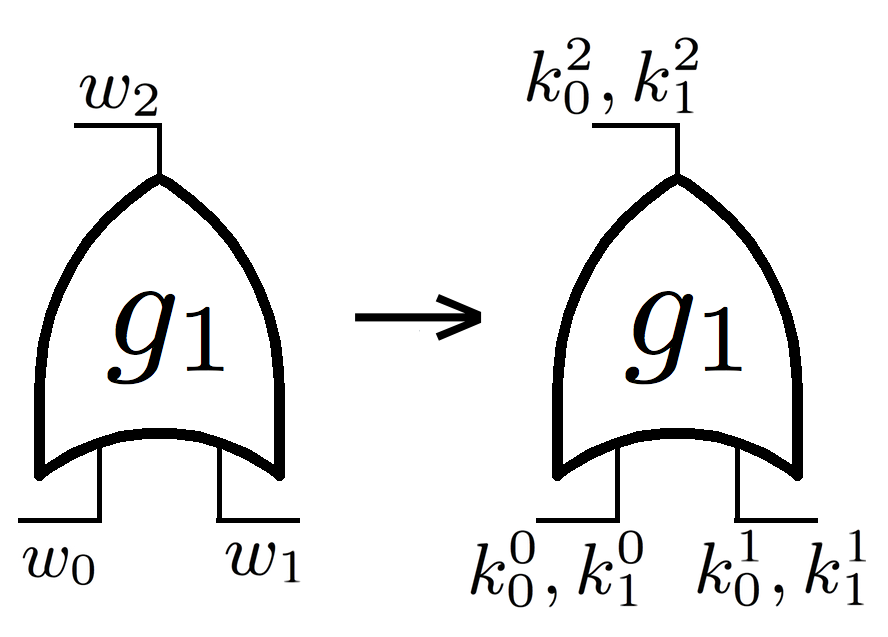
\includegraphics[width=\columnwidth]{images/or_gate}
    \caption{Garbling a single gate}
    \label{fig:garblegateimg}

    \subfloat[Original Values]{
        \begin{tabular}{ c | c || c }
            \hline
            $w_0$ & $w_1$ & $w_2$ \\
            \hline
            0 & 0 & 0 \\
            \hline
            0 & 1 & 1 \\
            \hline
            1 & 0 & 1 \\
            \hline
            1 & 1 & 1 \\
            \hline
        \end{tabular}
        \label{fig:gategarblepre}
    }
    \subfloat[Garbled Values]{
        \begin{tabular}{ c | c || c || c }
            \hline
            $w_0$ & $w_1$ & $w_2$ & garbled value \\
            \hline
            $k^0_0$ & $k^0_1$ & $k^0_2$ & $H(k^0_0 || k^0_1 || g_1) \oplus k^0_2$\\
            \hline
            $k^0_0$ & $k^1_1$ & $k^1_2$ & $H(k^0_0 || k^1_1 || g_1) \oplus k^1_2$\\
            \hline
            $k^1_0$ & $k^0_1$ & $k^1_2$ & $H(k^1_0 || k^0_1 || g_1) \oplus k^1_2$\\
            \hline
            $k^1_0$ & $k^1_1$ & $k^1_2$ & $H(k^1_0 || k^1_1 || g_1) \oplus k^1_2$\\
            \hline
        \end{tabular}
        \label{fig:gategarblepost}
    }
    \caption{Computation table for $g^{OR}_1$}
    \label{fig:gategarble}
\end{figure}

\begin{figure}[t!]
    \centering
    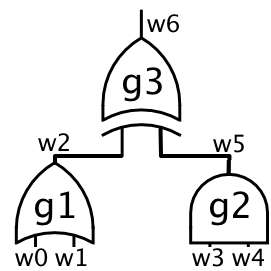
\includegraphics[width=\columnwidth]{images/multi_gates}
    \caption{Composing several gates into a simple circuit}
    \label{fig:garblecircuitimg}
    \subfloat[Original Values]{
        \begin{tabular}{ c | c || c }
            \hline
            $w_3$ & $w_4$ & $w_5$ \\
            \hline
            0 & 0 & 0 \\
            \hline
            0 & 1 & 0 \\
            \hline
            1 & 0 & 0 \\
            \hline
            1 & 1 & 1 \\
            \hline
        \end{tabular}
        \label{fig:andgatepre}
    }
    \subfloat[Garbled Values]{
        \begin{tabular}{ c | c || c || c }
            \hline
            $w_3$ & $w_4$ & $w_5$ & garbled value \\
            \hline
            $k^0_3$ & $k^0_4$ & $k^0_5$ & $H(k^0_3 || k^0_4 || g_2) \oplus k^0_5$\\
            \hline
            $k^0_3$ & $k^1_4$ & $k^0_5$ & $H(k^0_3 || k^1_4 || g_2) \oplus k^0_5$\\
            \hline
            $k^1_3$ & $k^0_4$ & $k^0_5$ & $H(k^1_3 || k^0_4 || g_2) \oplus k^0_5$\\
            \hline
            $k^1_3$ & $k^1_4$ & $k^1_5$ & $H(k^1_3 || k^1_4 || g_2) \oplus k^1_5$\\
            \hline
        \end{tabular}
        \label{fig:andgatepost}
    }
    \caption{Computation table for $g^{AND}_2$}
    \label{fig:andgate}

    \subfloat[Original Values]{
        \begin{tabular}{ c | c || c }
            \hline
            $w_2$ & $w_5$ & $w_6$ \\
            \hline
            0 & 0 & 0 \\
            \hline
            0 & 1 & 1 \\
            \hline
            1 & 0 & 1 \\
            \hline
            1 & 1 & 0 \\
            \hline
        \end{tabular}
        \label{fig:xorgatepre}
    }
    \subfloat[Garbled Values]{
        \begin{tabular}{ c | c || c || c }
            \hline
            $w_2$ & $w_5$ & $w_6$ & garbled value \\
            \hline
            $k^0_2$ & $k^0_5$ & $k^0_6$ & $H(k^0_2 || k^0_5 || g_3) \oplus k^0_6$\\
            \hline
            $k^0_2$ & $k^1_5$ & $k^1_6$ & $H(k^0_2 || k^1_5 || g_3) \oplus k^1_6$\\
            \hline
            $k^1_2$ & $k^0_5$ & $k^1_6$ & $H(k^1_2 || k^0_5 || g_3) \oplus k^1_6$\\
            \hline
            $k^1_2$ & $k^1_5$ & $k^0_6$ & $H(k^1_2 || k^1_5 || g_3) \oplus k^0_6$\\
            \hline
        \end{tabular}
        \label{fig:xorgatepost}
    }
    \caption{Computation table for $g^{XOR}_3$}
    \label{fig:xorgate}
\end{figure}

To see how \ac{P1} does this, first consider a single logical OR gate, $g^{OR}_1$, represented in figure \ref{fig:garblegateimg}. Initially \ac{P1} generates the values for this gate as normal, resulting in the truth table in figure \ref{fig:gategarblepre}. \ac{P1} then generates a key for each possible value for each wire in the gate.  This results in 6 keys being generated, one for each of the two possible boolean values on each of the three wires in the gate.

\ac{P1} then encrypts each entry in the table for the output wire using the keys used for the corresponding inputs.  The gate identifier serves as a nonce and is only included in this construction to ensure that the same values are never encrypted twice in the circuit.  \ac{P1} then randomly orders the rows the table, further obscuring the underlying boolean values\footnote{To simplify the presentation, this step is not shown in figure \ref{fig:garblegateimg}.}).

This encryption plays two important roles in the protocol.  First, since the output of each encryption operation is assumed be random (i.e. the hash function is assumed to perform like a random oracle), it removes any correlation between the underlying truth values in the table and the resulting garbled values. Even though this gate produces three identical boolean values, the garbled values all uniformly distributed, revealing nothing about the underlying value being encrypted.

Second, encrypting the output keys under the input keys prevents \ac{P2}, the circuit evaluator, from playing with the circuit and considering other inputs other than those provided by \ac{P1}. \ac{P2} can only obtain one of the output keys from the table, since she will only have, at most, the necessary input keys to the gate to decrypt one value for the output wire.

Once \ac{P1} has garbled the values for one gate, he can continue the process to compose an arbitrarily large circuit.  Figure \ref{fig:garblecircuitimg} shows how multiple garbled gates can be composed together into a simple circuit, and the how the keys from each gate are carried forward into the next gate, blinding the computing party from the learning the intermediate values being calculated.

The only gates in the circuit that do not need to be garbled are the output gates, or gates with wires that do not serve as input wires to another gate.  The output values from these gates can remain unobscured since they are outputting the final result of the circuit, a value which \ac{P2} is allowed to learn.


\subsubsection{Sending Garbled Values to \ac{P2}}

Once \ac{P1} has finished generating the garbled circuit, he then needs to garble his input to the function, creating a mapping of $i_{P1}$ to its garbled equivalents.  \ac{P1} begins this process by replacing the first bit of his input with the corresponding key for that input wire in the circuit.  For example, \ac{P1}'s first bit was input into $w_0$, and the value of $i^0_{P1}$ was 1, \ac{P1} would select $k^1_0$ to be the first value in his input to the garbled circuit. \ac{P1} then repeats this procedure for the remaining bits in his input, creating \ac{P1}'s garbled input. \ac{P1} then sends the garbled circuit $c_g$ and his garbled input to \ac{P2}.

\subsubsection{Receiving \ac{P2}'s Input Values through \ac{OT}}

\ac{P2} receives $c_g$ and \ac{P1}'s garbled input, but still needs the garbled representation of her own input to compute the circuit. Recall that \ac{P1} has the garbled values for all of \ac{P2}'s input wires, but has no knowledge of what values correspond to \ac{P2}'s true input. \ac{P2}, inversely, knows the bits of her own input, but not the corresponding keys for her input wires in $c_g$.

\ac{P2} maps the first bit of her input to its corresponding garbled value by engaging in \emph{1-out-of-2 \ac{OT}}s with \ac{P1}, where \ac{P1}'s inputs are $(k^0_1, k^1_1)$, and \ac{P2}'s input is 0 or 1, depending on the first bit of \ac{P2}'s input.  \ac{P2} performs additional \ac{OT}s with \ac{P1} for all values $0 < i < |i_{P2}|$ to achieve her full garbled input into $c_g$.

\subsubsection{Computing the Garbled Circuit}

Once \ac{P2} has both garbled inputs and the garbled circuit, she can straight forwardly compute the circuit.  For each input gate, \ac{P2} looks up the corresponding value from \ac{P1} and \ac{P2}'s garbled input values and uses them as keys to decrypt the output value from the gate's garbled truth table.  Since \ac{P2} does not know which output key these two input keys correspond to, \ac{P2} must try to decrypt each of the four output keys.  If the protocol has been carried out correctly, only one of the four values will decrypt correctly.  The other three decryption attempts will produce $\bot$. The newly decrypted key then becomes an input key to the next gate.

\ac{P2} continues this process until she reaches the output wires of the circuit.  Each of these wires output a single, unencrypted bit.  \ac{P2} then reassembles the output bits and has the correct solution for the \ac{f} encoded by $c_g$.  \ac{P2} completes the protocol by sending the output of the circuit to \ac{P1}.

\section{Protocol Security}
\label{sec:security}

Yao's protocol is designed to provide \ac{SFE} against \emph{semi-honest} adversaries. These security guarantees do not carry over against \emph{malicious} adversaries though.  This is a serious shortcoming for being able to make the protocol practical; there are relatively few real-world scenarios where you do not trust the other party to see your inputs to a function, but do trust them to forgo the opportunity to discover those same inputs by deviating from the protocol.

Much work has been conducted to extend Yao's protocol to be secure against \emph{malicious} adversaries.  This work can generally be classified into three areas, 1) creating \emph{1-out-of-2 \ac{OT}} protocols that are secure against \emph{malicious} adversaries, 2) ensuring that the circuit constructing party correctly constructs the garbled circuit, and 3) preventing \ac{P1} from gaining an advantage by sending \ac{P2} corrupt values for her input.

\subsection{Securing the \ac{OT} Protocol}
\label{sec:securingot}

The \emph{1-out-of-2 \ac{OT}} protocol described in the section \ref{sec:ot} is trivially vulnerable in the \emph{malicious} case.  Instead of generating $((k^{pub}_b, k^{pri}_b), (k^\bot_{b-1}, \bot))$, \ac{P2} could easily generate two valid public / private key pairs, allowing her to recover both values sent by \ac{P1}. Applied to Yao's protocol, this would allow \ac{P2} to learn both the garbled versions of the 0 and 1 values for all of her input bits. \ac{P2} having these additional keys would allow \ac{P2} to decrypt additional values throughout the circuit garbled gate, violating the \emph{privacy} requirement of \ac{SFE}.  Others have detailed several additional ways that using an insecure-in-the-\emph{malicious}-case, \ac{OT} protocol can be exploited by an attacker\cite{kiraz2006protocol}.

As previously discussed, \ac{OT} is a distinct, though related, field to \ac{SFE} in general and Yao's protocol in particular.  As such, this section does not attempt to assess the state of the art of in the field of \ac{OT}.  A variety of other approaches to \emph{malicious}-case secure \emph{1-out-of-2 \ac{OT}} protocols exist\cite{naor2001efficient, kiraz2006protocol, goldreich1987play, naor2005computationally}, each with their own tradeoffs, computation cost and underlying security assumptions.  The below protocol\cite{bellare1990non}\footnote{This protocol is a slightly modified version of the protocol presented in \cite{bellare1990non}, to incorporate a change suggested by \cite{naor2001efficient} to remove the reliance on a external zero knowledge proof or other out-side-the-protocol source for \emph{C}.} is included to show that efficient \emph{1-out-of-2 \ac{OT}} is possible, and that researchers have used it and equivalent \ac{OT} protocols to make Yao's \ac{GCP} secure in the \emph{malicious} case.

\begin{algorithm}[H]
    \floatname{algorithm}{Protocol}
    \caption{Malicious-Secure 1-out-of-2 Oblivious Transfer}
    \label{alg:otmalicious}
    \begin{algorithmic}[1]
        \STATE \ac{P1} has a set of two strings, $S = \{s_0, s_1\}$.
        \STATE \ac{P1} (sender) and \ac{P2} (receiver) agree on some $q$ and $g$ such that $g$ is a generator for $\mathbb{Z}^*_q$.
        \STATE \ac{P1} selects a random $C$ from $\mathbb{Z}^*_q$, or more generally such that \ac{P2} does not know the discrete log of $C$ in $\mathbb{Z}^*_q$.
        \STATE \ac{P2} selects $i \in \{0, 1\}$ corresponding to whether \ac{P2} wants $s_0$ or $s_1$. \ac{P2} also selects a random $0 \leq x_i \leq q-2$.
        \STATE \ac{P2} sets $\beta_i = g^{x_i}$ and $\beta_{i-1} = C \bullet (g^{x_i})^-1$. $(\beta_0, \beta_1)$ and $(i, x_i)$ form \ac{P1} public and private keys, respectively.

        \STATE \ac{P1} checks the validity of \ac{P2}'s public keys by verifying that $\beta_0 \bullet \beta_1 = C$.  If not, \ac{P1} aborts.

        \STATE \ac{P1} selects $y_0, y_1$ such that $0 \leq y_0, y_1 \leq q-2$, and sends \ac{P2} $a_0 = g^{y_0}, a_1 = g^{y_1}$.
        \STATE \ac{P1} also generates $z_0 = \beta^{y_0}_0, z_1 = \beta^{y_1}_1$ and sends \ac{P2} $r_0 = s_0 \oplus z_0$ and $r_1 = s_1 \oplus z_1$.
        \STATE \ac{P2} computes $z_i = a^{xi}_i$ and then receives $s_i$ by computing $s_i = z_i \oplus r_i$.
    \end{algorithmic}
\end{algorithm}

The purpose of many of the steps in the protocol are not explicit in the original work\cite{bellare1990non}, so some context is added here.  Specifically, in step 5 \ac{P1} checks that $\beta_0 \bullet \beta_1 = C$ to prevent \ac{P2} from being able to decrypt under both $\beta_0$ and $\beta_1$, to force \ac{P2} to choose one or the other. As long as the assumption that \ac{P2} does not know the discrete log of $C$ holds, then it follows that \ac{P2} cannot know the discrete log of both $\beta_0$ and $\beta_1$.

% Similarly, steps 7, 8 and 9 function similarly to a Diffie-Hellman key exchange.  In step 8, it will either be the case that $z_0 = \beta^{y_0}_0
%  = g^{{x_i}^{y_0}} = g^{x_i \bullet y_0}$ or $z_1 = \beta^{y_1}_1
%  = g^{{x_i}^{y_1}} = g^{x_i \bullet y_1}$, depending on \ac{P2}'s choice for $i$. This allows \ac{P2} to generate either

% in steps 7 and 8, note that either $a_0$ or $a_1$ will be equal to the \ac{P2} selected $\beta_i$.

\subsection{Securing Circuit Construction}
\label{sec:securingcircuits}

A second way a malicious adversary could exploit Yao's protocol to learn information about the other party's input is by \ac{P1} creating and garbling a circuit for a function other than the function expected by \ac{P2}. Trivially, \ac{P1} could send \ac{P2} a garbled circuit couple simply send \ac{P2}'s input to \ac{P1}, or leak information about $i_{P2}$ in some other manner not known by \ac{P2}.  It is therefor necessary for \ac{P2} to ensure that the garbled circuit she computes is actually a garbled representation of the expected function.

\subsubsection{Zero-Knowledge Proofs}

Two different general strategies for achieving this assurance have been promoted.  The first approach is that \ac{P1} generates a zero knowledge proof of the garbled circuit's correctness, and then sends this proof to \ac{P2} along with the garbled circuit and \ac{P1}'s garbled inputs\cite{goldreich1987play, goldreich2009foundations}.

This zero-knowledge strategy dates back to earlier in this history of Yao's protocol, when the protocol was treated as proof that \ac{SFE} was possible, instead of as a practical tool for actually achieving \ac{SFE}. More recent, implementation-focused work on Yao's protocol has treated the zero-knowledge proof approaches as too expensive for practical use\cite{lindell2007efficient, mohassel2006efficiency, malkhi2004fairplay}.

\subsubsection{Cut-and-Choose}

Instead, recent work on Yao's protocol has focused on a \emph{cut-and-choose} strategy for securing circuit construction\cite{malkhi2004fairplay}. Work on this approach has developed in an arms-race fashion, with proposals being made, other researchers revealing shortcomings in the given strategy, and a new strategy being developed to address the given short coming. Several rounds of this propose-attack-revise cycle are discussed below, to give context and meaning to each proposed improvement.\\[.5em]

\noindent\textbf{Standard Cut-and-Choose}

Under this approach, \ac{P1} constructs $m$ versions of the circuit, each structured the same but garbled so that the keys for each gate in the circuit are all unique. \ac{P1} does the same for his inputs to each of the garbled circuits. Additionally, \ac{P1} generates a commitment for each of his garbled inputs, which for simplicity can be represented by a simple hash function.\footnote{Tough several more secure methods of committing are mentioned in \cite{lindell2007efficient}, a simple hash function is used here to simplify the description of the cut-and-choose approach.  A more secure approach is described here \cite{halevi1996practical}},

\ac{P1} then sends each of these pairs of garbled circuits and associated input commitments to \ac{P2}, who selects $m-1$ versions of the circuit to verify.  \ac{P1} de-garbles each of the $m-1$ selected circuits, so that \ac{P2} can see the underlying circuit with the obscured boolean values in each gates' computation table.  \ac{P2} can then verify that each of the revealed circuits is constructed correctly.

If everything looks correct to \ac{P2} she will continue with the computation by receiving \ac{P1} garbled inputs, checking that they match the previously sent commitment (again, most simply thought of as checking that the hash of the received garbled inputs matches the previously sent hash), and then proceed with Yao's protocol as normal. This reduces the chances of \ac{P1} tricking \ac{P2} into computing a corrupted circuit to $1/m$. This protocol is provided more formally in Protocol \ref{alg:cutandchoose-basic}.

\begin{algorithm}[H]
    \floatname{algorithm}{Protocol}
    \caption{Securing Circuit Construction With Cut-and-Choose}
    \label{alg:cutandchoose-basic}
    \begin{algorithmic}[1]
        \STATE \ac{P1} generates $m$ garbled versions of the circuit $c$, along with a corresponding garbled version of his input, called $X_i$ for $0 \leq i < m$.
        \STATE \ac{P1} uses hash function $H$ to generate commitments to each garbled input, $COMMIT_i = H(X_i)$ for $0 \leq i < m$.

        \STATE \ac{P1} sends \ac{P2} $m$ garbled circuits and $COMMIT$ such that $|COMMIT| = m$.
        \STATE \ac{P2} selects $0 \leq j < m$ and \ac{P1} un-garbles all circuits except the $j$th.
        \STATE \ac{P2} inspects all $m-1$ circuits to check that they are correctly formed. If not, \ac{P2} aborts.

        \STATE \ac{P2} receives \ac{P1}'s garbled inputs to circuit $j$ and confirms that \ac{P1} did not change his inputs by verifying $COMMIT_j = H(X_j)$. If not, \ac{P2} aborts.

        \STATE Otherwise, \ac{P2} receives the continues with Yao's protocol as normal.
    \end{algorithmic}
\end{algorithm}


\noindent\textbf{Further Securing Cut-and-Choose}

However, for many applications one may wish for a stronger guarantee against executing a malicious circuit from \ac{P1}.  Lindell and Pinkas\cite{lindell2007efficient} discovered that \ac{P1}'s odds of success can be dramatically reduced without the overhead of needing to generate additional circuits by altering the cut-and-choose strategy slightly.

Instead of \ac{P2} having \ac{P1} reveal $m-1$ circuits, Lindell and Pinkas have \ac{P2} select only $m/2$ circuits to be revealed.  \ac{P2} computes the remaining $m/2$ circuits and takes the majority result. Under this construction, a malicious \ac{P1} would only succeed in having \ac{P2} output the result of a corrupt circuit if a) \ac{P1} constructed more than $1/4$ of the circuits to be corrupt, and b) none of those corrupt $m/4$ circuits were among the $m/2$ circuits \ac{P2} selected to be revealed.  Lindell and Pinkas measure \ac{P1}'s chance of success in such an attack at $2^{-0.311m}$, where $m$ is the number of circuits generated\cite{lindell2007efficient}.\\[.5em]

\noindent\textbf{Majority Result as a Defense Against a Malicious Circuit}

An immediate question that comes out of the above approach is why \ac{P2} should take the majority result of the computed $m/2$ circuits, instead of immediately aborting when encountering the first corrupt circuit, especially given that computing a garbled circuit is a very expensive operation.  The reason is that, were \ac{P2} to abort if all circuit outputs were not identical, she would become vulnerable to a different attack from \ac{P1}.

Consider the case where \ac{P1} constructs all circuits correctly, with a single exception.  This corrupt circuit outputs the correct value of the function $\oplus$'ed with the first bit of \ac{P2}'s input.  By observing whether \ac{P2} finishes computing all still-garbled $m/2$ circuits, \ac{P1} is able to learn the first bit of \ac{P2}'s input.

\begin{figure}[t]
    \centering
    \begin{tabular}{ c | c | c | c | l }
        \hline
        $f_0$ & $i_{P2_0}$ & $f_0 \oplus i_{P2_0}$ & \ac{P2} returns & \ac{P1} learns \\
        \hline
        0 & 0 & 0 & 0 & $i_{P2_0} = 0$\\
        \hline
        0 & 1 & 1 & $\bot$ & $i_{P2_0} = 1$\\
        \hline
        1 & 0 & 1 & 1 & $i_{P2_0} = 0$\\
        \hline
        1 & 1 & 0 & $\bot$ & $i_{P2_0} = 1$\\
        \hline
    \end{tabular}
    \caption{Using a corrupted circuit to learn first bit of \ac{P2}'s input}
    \label{fig:earlyabortattack}
\end{figure}

Figure \ref{fig:earlyabortattack} provides a full explanation of how \ac{P1} performs this attack.  The first column depicts the first bit of the correct value returned by $f$, and the second column shows the first bit of \ac{P2}'s input.  The third column shows the value returned by \ac{P1}'s single malicious circuit, and column four describes the value \ac{P2} returns from evaluating the entire $m/2$ set of circuits (or $\bot$ if \ac{P2} aborts).  Finally, column five shows what \ac{P1} is able to learn about \ac{P2}'s input, without having access to the first three columns of the table.


\subsection{Securing Against Corrupt Inputs}

A third area where a malicious party can exploit the original construction of Yao's protocol is in the values \ac{P1} chooses to return to \ac{P2} in the \emph{1-out-of-2 \ac{OT}} step.  Recall that this \ac{OT} step is taken to prevent \ac{P1} from learning whether \ac{P2} is requesting the garbled value for a 0 or a 1 bit in her input.  The protections given in the previous two subsections provide no security against this attack. Subsection \ref{sec:securingot} only addresses ensuring that \ac{P1} cannot learn \ac{P2}'s inputs during the \ac{OT} step, not that these inputs cannot be leaked elsewhere in the protocol.  Similarly, subsection \ref{sec:securingcircuits} provides \ac{P2} guarantees that the circuits being evaluated are not corrupt, but provides no guarantees against corrupt inputs.

\ac{P1} can obtain information about \ac{P2}'s inputs by returning a corrupt value to \ac{P2} during the \ac{OT} step in the protocol.  \ac{P1} carries out the attack works as follows.  Instead of returning the correct garbled values for the 0 and 1 values of \ac{P2}'s input, \ac{P1} returns the correct garbled value for 0, and a corrupt value for 1.  \ac{P1} can then learn whether \ac{P2} received the 0 or 1 value by observing if \ac{P2} aborts while computing the circuit.  If \ac{P2} received the 0 value, she will be able to compute the circuit as normal.  However, if \ac{P2} received the 1 value, she will not be able to compute the circuit and will be forced to abort.  Either way, \ac{P1} is able to learn the value of a bit of \ac{P2}'s input.

\begin{figure}
    \centering
    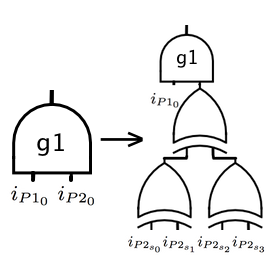
\includegraphics[width=\columnwidth]{images/secureing_malicious_inputs}
    \caption{Securing against \ac{P1} providing malicious inputs through s new $\oplus$ gates}
    \label{fig:inputsecure}
\end{figure}

A defense against this attack was also given by Lindell and Pinkas\cite{lindell2007efficient} and show in figure \ref{fig:inputsecure}.  They secure the protocol by adding $s|i_{P2}|$ input bits to the circuit, where $s$ is a chosen security parameter.  Each of \ac{P2}'s input bits is replaced by an $\oplus$ing of $s$ new input bits, each chosen by \ac{P2} from \ac{P1} through the same \ac{OT} protocol.  The circuit is also augmented to reflect these new input bits and $\oplus$ gates. This step of indirection gives \ac{P2} $2^{s-1}$ ways to receive the each of her true input bits from \ac{P1}, and prevents     \ac{P1} from learning the underlying input bit by corrupting the augmented, $\oplus$ed inputs.  Note that this construction does not prevent \ac{P1} from forcing \ac{P2} to abort when executing the circuit, it only prevents \ac{P1} from learning anything about \ac{P2}'s input.


\section{Protocol Performance}
\label{sec:performance}

Yao's protocol gives a polynomial time solution for the \ac{SFE} problem, both in the \emph{semi-honest} and \emph{malicious} cases (once the adjustments made in section \ref{sec:security} are made).  However, while Yao's protocol is by this definition ``efficient'', it is also costly, and for many problems prohibitively so.  For example, Kreuter, shelat and Shen\cite{kreuter2012billion} found that computing the edit distance of two 4095-bit strings required a circuit of over 5.9 billion gates, even given with a highly optimized circuit.

A great deal of work has been done to make the protocol less expensive to execute.  This work broadly falls into three categories: 1) communication cost optimization that reduce the communication cost of the protocol by minimizing the amount of information that must be shared between the two parties, 2) execution optimizations that that allow for the same number of gates to be executed in a shorter amount of time, and 3) circuit optimizations that reducing the number of gates needed to compute the function.

Optimizations do not always cleanly fall into only one of these categories, and improvements in one area often have spill over benefits in another.  For example, reducing the number of gates needed to compute a circuit also reduces the number of gates that need to be communicated between parties.  The following categorization is more meant to provide an intuition about the main role of each optimization, and less a strict taxonomy of contributions.


\subsection{Communication Optimizations}

The communication costs of transmitting a garbled circuit from \ac{P1} to \ac{P2} dwarfs all other communication related costs in Yao's protocol\footnote{For all but the most trivial functions.}.  To see why, recall that circuits can grow to contain billions of gates, and that each wire connecting each of these gates is represented by four multi-byte strings, meaning each garbled circuit can be gigabytes in size. This problem is made worse when considering the protocol in the \emph{malicious} setting, where the \emph{cut-and-check} strategy requires \ac{P1} to send many copies of the garbled circuit to \ac{P2}. Minimizing the amount of information that must be communicated between the parties in the protocol is therefor a significant issue in making Yao's protocol practical.

\subsubsection{Random Seed Checking}

A solution to this problem was presented by Goyal, Mohassel and Smith\cite{goyal2008efficient}. Their technique significantly reduces the communication costs of Yao's protocol in two steps.

First, instead of having \ac{P1} assign values for each wire in the circuit randomly, \ac{P1} selects a random seed for each garbled version of the circuit, then uses that random seed to deterministically generate each of the the random values used in the circuit.

Second, instead of sending \ac{P2} $m$ copies of the garbled circuit during the \emph{cut-and-check} phase, \ac{P1} instead sends \ac{P2} ``commitments'' for each version of the circuit.  \ac{P2} then chooses $m/2$ circuits for \ac{P1} to reveal.  \ac{P1} then sends \ac{P2} the random seed used for each selected circuit, along with any structural information \ac{P2} needs to generate the garbled circuit from the random seed.

Once \ac{P2} has verified that the revealed circuits are correct, she then checks that \ac{P1}'s commitments for each circuit are correct (loosely, by hashing each random-seed generated circuit and seeing if it matches the corresponding commitment).  Finally, \ac{P1} sends \ac{P2} the remaining $m/2$ circuits for \ac{P2}'s evaluation.

This technique reduces the communication overhead of the protocol by approximately $1/2$, since the commitments \ac{P1} sends are constant in size and much much smaller than the size of a circuit.


\subsection{Execution Optimizations}

This subsection describes several techniques that have been discovered to allow parties to more quickly compute secure versions Yao's protocol without needing to significantly change how the circuit is stored or how information is shared between the two parties.  These other techniques are discussed in later subsections.

\subsubsection{Fast Table Lookups}

The \emph{fast table lookups}\footnote{The name of this technique comes from\cite{huang2011faster}, though versions of it are in work at least as early as\cite{malkhi2004fairplay}, if not earlier.} technique speeds up \ac{P2}'s evaluation of a circuit by removing the need for \ac{P2} to attempt to decrypt each row of each gate's garbled truth table until she finds a value that decrypts correctly.  Instead, the circuit constructor adds an additional bit to the end of each garbled output value. This additional bit serves as half of an index into the next gate's garbled truth table. Since each each garbled truth table contains four output values, and each gate has two input wires (each with one index bit), combining the index bits from both input values can uniquely identify which of the four values in the gate's garbled truth table the input values decrypt.

Note that since the order of the rows each garbled truth table is randomized during construction, these index values do not reveal any information about the underlying values, and thus do not affect the security of the the system.

\subsubsection{Pipelined Circuit Execution}

Garbled representations of circuits computing even simple functions can grow extremely large, making them difficult to store in memory for both the generating and computing party, as well as time consuming to generate (since \ac{P2} is waiting idle while \ac{P1} is garbling the circuit).  Huang, Evans, et al.\cite{huang2011faster} realized that the garbling and executing processes could be partially conducted in parallel, with \ac{P1} sending \ac{P2} the garbled gates as quickly as he is able to encrypt them, and \ac{P2} continuing to compute as long as she has at least gate to compute for which she has inputs for.

This technique has two benefits.  It prevents either party from needing to keep an entire circuit in memory (though the optimal strategy for minimizing the working set needed in memory is an open problem\cite{kreuter2012billion}), and it roughly reduces the time needed to compute a garbled circuit from $t_{garble} + t_{OT} + t_{evaluate}$ to $max(t_{garble}, t_{evaluate}) + t_{OT}$.

The above construction works in the \emph{semi-honest} context, but does not carry over to the \emph{malicious} case, since \ac{P1} would need to hold copies of each of the $m$ constructed circuits for

%             * Kreuter, shelat, Shen, "Billion-Gate Secure Computation with Malicious Adversaries" [2012]
%                 - Technique could also be used allow for piplined circuit generation and execution, though only in the semi-honest model, since all circuts need to be completed and hashed before any cut and choose operations can be executed, and thus before any circuits can be executed.

%                   - Ie the Huang method does not work with the random seed strategy
%                 - Extension of Huang et al aproach to allow for parallelized execution by having generator generate all circuits twice, before coin-toss / check-circuit selection to generate hash values, and afterwards to produce all circuits (for execution and checking)
\subsection{Circuit Optimizations}

A straight forward way of reducing the cost of Yao's protocol is to reduce the size of the garbled gates that must be evaluated. This section discusses several strategies that have been used to reduce the number of gates needed to compute the same function.

\subsubsection{Circuit Simplification}

Reducing the number of gates in the pre-garbled circuit trivially reduces the number of garbled gates that need to be evaluated later on.  This can be though of as a preprocessing stage that optimizes the circuit before garbling it.  Put another way, this state attempts to remove inefficiencies introduce when the underlying circuit was being encoded as a circuit.

Circuit optimization strategies include looking for unused gates, or gates that have no effect on the circuit, finding sub-circuits that can be more efficiently represented by a smaller number of gates, and removing identity gates and sub-circuits, or sets of gates who are guaranteed to evaluate to 0 or 1\cite{kreuter2012billion, pinkas2009secure}.  The benefit of from this type of optimization will be inversely related to the quality of circuits generated by the function-to-circuit translating process.  One study\cite{pinkas2009secure} found a 60\% reduction in circuit size when optimizing circuits generated from a well known circuit generator\cite{malkhi2004fairplay}.


\subsubsection{Free XOR Optimization}

A second strategy for reducing the number of gates needed in a garbled circuit comes form the free XOR strategy, discovered by Kolesnikov and Schneider\cite{kolesnikov2008improved}.  This optimization allows for the circuit constructor to replace all garbled XOR gates in the circuit with a simple XOR operations. This results in the significant improvement of removing four encrypted values from the circuit for every XOR gate.

The free XOR technique works by changing how some of the garbled values for wires in the circuit are selected. Recall that by default each garbled value of 0 and 1 for each wire in the circuit is selected randomly.  The free XOR technique instead relates the values of the input wires to XOR gates so that the gate's correct output values can be computed with a single XOR operation, instead of needing to look up the output value in a garble truth table. Since garbled truth tables are no longer needed for all XOR gates, the size of the garbled circuit is reduced by $|XOR gates| \bullet |k|$, where $k$ is the size of the garbled values used in the circuit. The free XOR technique is described more formally in algorithm \ref{alg:freexor}.

\begin{algorithm}[H]
    \floatname{technique}{Algorithm}
    \caption{Free XOR Technique}
    \label{alg:freexor}
    \begin{algorithmic}[1]
        \STATE \ac{P1}, the circuit constructor, generates secret $R = r||1$ where $r \in \{0, 1\}^{k-1}$.
        \STATE Let $X$ be the set of all XOR gates in the circuit, and let $g_{in_0}$ and $g_{in_1}$ refer to the gates in the circuit who's output wires serve as the input wire to gate $g$. Finally, let $k^b_{in_i}$ refer to the $b \in \{0, 1\}$ value of wire leaving $g_{in_i}$ and entering $g$.
        \FOR {$g \in X$}
            \STATE Set $k^1_{in_0} =  R \oplus k^0_{in_0}$ and $k^1_{in_1} =  R \oplus k^0_{in_1}$.
            \STATE Replace $g$ with a function returning $k_{in_0} \oplus k_{in_1}$.
        \ENDFOR
    \end{algorithmic}
\end{algorithm}


\subsubsection{Garbled Row Reduction}


%         - Garbled Row Reduction
%             * Pinkas, Schneider, Smart, Williams "Secure Two-Parry Computation is Practical" [2009]
%             - Remove one entry in garbling tables from AND and OR gates by… (gotta figure this one out)


\section{Implementations}
\label{sec:implementations}

\section{Conclusion}
\label{sec:conclusion}

This paper attempted to provide an overview of the field of \ac{SFE} using Yao's garble circuits protocol.  In addition to the techniques and approaches discussed in this paper, there is a great deal of related work in other fields that might be of interest for those interested in practical \ac{SFE}, such as zero-knowledge proof systems, performance optimizing \ac{OT} constructions, malleable claw-free collections, and verifiable secret sharing.



\bibliographystyle{abbrv-firstname-plainnat}
\bibliography{combined}

%\balancecolumns
\end{document}
